
\chapter{Description de l'application mobile}\label{ch:app_mobile}

L'application mobile, aussi appelé RaceTracker dans ce document, permet de visualiser, en temps réel, les informations produites par les capteurs porté par les sportifs. En plus de cela elle permet également d'administrer les compétitions.

Elle est codée en langage Java et utilise le système Android et également le "Maps SDK for Android" de Google qui permet d'interagir avec les cartes ce qui permet l'ajout de marqueurs ou de dessiner des formes géométriques par exemple.

L'environnement de développement Android Studio a été utilisé pour le développement de cette application qui permet également de simuler l'exécution de l'application et facilite ainsi le débuggage.

\todo{Image GUI}

\section{Architecture logiciel}

L'architecture logiciel de l'application mobile est présenté ci-dessous. Une application Android est composée de "Activities", qui représentent chacun des écrans disponibles dans l'application. Des "Fragments" sont également utilisés, ce sont des morceaux d'interface graphique qui peuvent être insérer dans des "Activities". Enfin l'application mobile utilise des classes qui sont responsable de la gestion de l'application et de l'accès à la base de données.

La figure \ref{fig:app_static_archi} présente l'architecture statique de l'application mobile Android.

\begin{figure}[htb]
\centering 
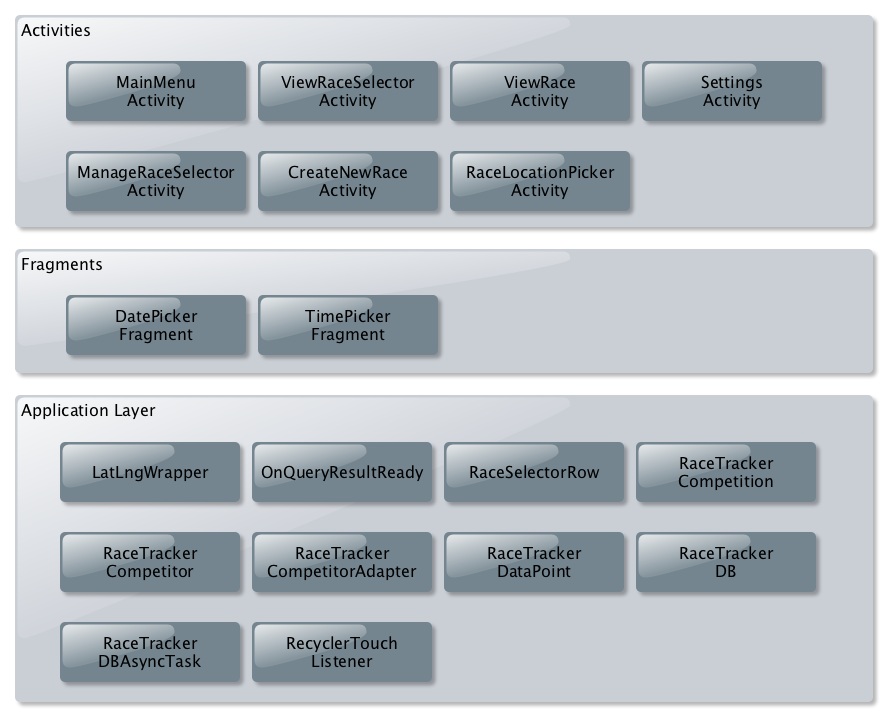
\includegraphics[width=1\columnwidth]{app_static_archi.png} 
\caption{Architecture statique de l'application mobile}
\label{fig:app_static_archi}
\end{figure}

Durant l'exécution de l'application mobile, le thread principal est entièrement géré par le système d'exploitation Android, il est en charge de la mise à jour de l'interface graphique et de tout ce qui en est en lien comme par exemple le changement d'activité lors de l'appui d'un bouton par exemple. Lorsque l'application désire envoyer des requêtes à la base de données, elle utilise la classe RaceTrackerDBAsyncTask qui hérite de AsyncTask. Cette classe permet d'effectuer une tâche en arrière plan de manière asynchrone et de gérer le résultat une fois la tâche terminée. Enfin lorsque l'utilisateur est en train de visionner une course, un objet de type Handler est utilisé pour faire la requête du dernier point de donnée à intervalle régulier.

La figure \ref{fig:app_dyn_archi} montre l'architecture dynamique de l'application mobile. 

\begin{figure}[htb]
\centering 
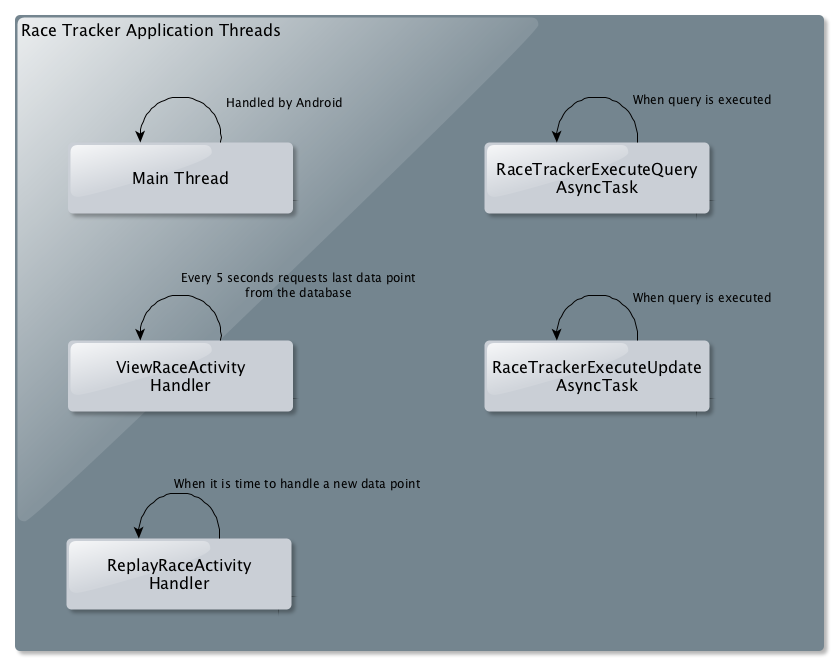
\includegraphics[width=1\columnwidth]{app_dyn_archi.png} 
\caption{Architecture dynamique de l'application mobile}
\label{fig:app_dyn_archi}
\end{figure}

\section{Les librairies externes}

L'application mobile utilise principalement deux librairies externes, la première est le "Maps for Android SDK", cette librairie permet d'ajouter à son application mobile une carte de type google maps et d'interagir avec elle. Elle permet d'ajouter des marqueurs à des position (latitude/longitude) spécifiques, de créer des lignes entre les points ou encore de modifier le comportement de la carte. La librairie est disponible sur \url{https://cloud.google.com/maps-platform/}.

Un exemple d'utilisation est proposé ci-dessous.

\todo{Add biblio}

\begin{lstlisting}[style=JavaStyle]
...
private GoogleMap mMap;

protected void onCreate(Bundle savedInstanceState) {
	/* Retrieve the map fragment when the map is ready */
	MapFragment mapFragment = (MapFragment) getFragmentManager().findFragmentById(R.id.mapView);
	mapFragment.getMapAsync(this);
}

@Override
public void onMapReady(GoogleMap googleMap) {
	mMap = googleMap;

	/* Change map type */
	mMap.setMapType(GoogleMap.MAP_TYPE_SATELLITE);

	/* Add a marker in Sydney, Australia */
	LatLng sydney = new LatLng(-34, 151);
	mMap.addMarker(new MarkerOptions().position(sydney).title("Marker in Sydney"));

	/* Move camera and zoom */
	mMap.moveCamera(CameraUpdateFactory.newLatLngZoom(sydney, -12));
}
...
\end{lstlisting}

La deuxième librairie externe utilisée et un driver de type JDBC permettant de s'interfacer avec une base de données PostgreSQL. C'est grâce à ce composant que l'application mobile va interroger la base de données afin de récupérer la liste des compétiteurs, les données relatives aux compétitions ou encore les points de données à afficher sur la carte. Le driver JDBC est téléchargeable gratuitement à l'adresse \url{https://jdbc.postgresql.org/}.

\begin{lstlisting}[style=JavaStyle]
...
public ResultSet executeQuery(String connection, String user, String password, String query) {
	Statement st;
	ResultSet results

	Connection conn = DriverManager.getConnection(connection, user, password);
	st = conn.createStatement();
	
	results = st.executeQuery(query);
	st.close()	
	
	return results;
}

public void myQuery() {
	String myQuery = "SELECT * FROM my_table;";
	ResultSet results;
	
	results = executeQuery("jdbc:postgresql://192.168.1.4:5432/mydatabase", "me", "1234", myQuery);
	
	while (results.getResult().next()) {
		System.out.println("Field test1: " + results.getString("field_test_1"));
		System.out.println("Field test2: " + results.getInt("field_test_2"));
	}
	
	results.close();	
}
...
\end{lstlisting}

\section{Les classes}

L'application mobile RaceTracker est composée de plusieurs class qui lui permettent d'effectuer ses tâches. Elles sont décrites dans cette section.

\subsection{MainMenuActivity}

L'activité principale de l'application, c'est le premier écran qui se lance et qui permet de choisir si l'on souhaite visionner une course ou alors faire des opérations d'administration sur la base de donnée. Lorsque l'utilisateur à fait son choix, elle lance l'activité suivante c'est à dire soit ViewRaceSelectorActivity ou ManageRaceSelectorActivity.

La figure \ref{fig:mainmenuactivity_uml} montre le diagramme de classe de MainMenuActivity.

\begin{figure}[htb]
\centering 
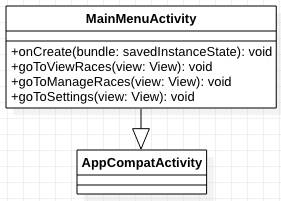
\includegraphics[width=0.4\columnwidth]{mainmenuactivity_uml.png} 
\caption{Diagramme de classe de MainMenuActivity}
\label{fig:mainmenuactivity_uml}
 \end{figure}

\todo{Image}

\subsection{ViewRaceSelectorActivity}

Cette activité permet à l'utilisateur de sélectionner la course qu'il souhaite visionner, lorsqu'elle se lance elle va allez interroger la base de données afin de récupérer la liste de toutes les compétitions et l'afficher à l'utilisateur qui peut ensuite décider, en cliquant sur l'objet de son choix, de visionner la course. Après avoir sélectionner la course, l'activité transfert le contrôle à ViewRaceActivity.

La figure \ref{fig:viewraceselector_uml} montre le diagramme de classe de ViewRaceSelectorActivity.

\begin{figure}[htb]
\centering 
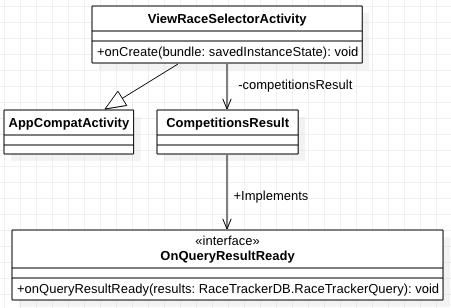
\includegraphics[width=0.6\columnwidth]{viewraceselector_uml.png} 
\caption{Diagramme de classe de ViewRaceSelectorActivity}
\label{fig:viewraceselector_uml}
 \end{figure}

\todo{Image}

\subsection{ViewRaceActivity}

Lorsque l'utilisateur désire regarder une course, c'est cette activité qui va être lancé. Elle est responsable de la gestion de l'affichage des informations sur la carte et également de la liste des compétiteurs. Périodiquement cette activité va allez chercher dans la base de données les points de données relatif à une course et vérifier si de nouveau points ont été ajouté auquel cas elle met à jour la carte avec la nouvelle position. Toutes ses informations sont récupérés depuis la base de donnée.

La figure \ref{fig:viewraceactivity_uml} montre le diagramme de classe de ViewRaceActivity.

\begin{figure}[htb]
\centering 
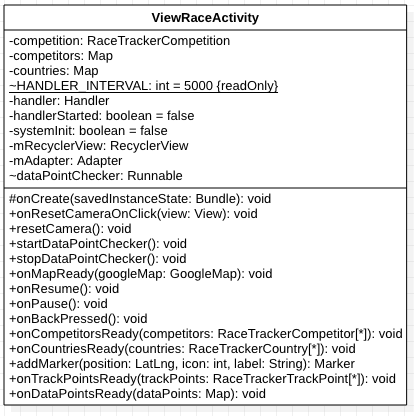
\includegraphics[width=0.8\columnwidth]{viewraceactivity_uml.png} 
\caption{Diagramme de classe de ViewRaceActivity}
\label{fig:viewraceactivity_uml}
 \end{figure}

\todo{Image}

\subsection{SettingsActivity}

Cette classe est en charge de la gestion de l'affichage du menu des paramètres. L'utilisateur peut modifier les paramètres relatifs à l'application grâce au menu proposé par cette activité.

La figure \ref{fig:settingsactivity_uml} montre le diagramme de classe de SettingsActivity.

\begin{figure}[htb]
\centering 
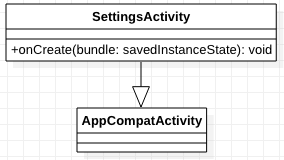
\includegraphics[width=0.4\columnwidth]{settingsactivity_uml.png} 
\caption{Diagramme de classe de SettingsActivity}
\label{fig:settingsactivity_uml}
 \end{figure}

\todo{Image}

\subsection{ManageRaceSelectorActivity}

La classe ManageRaceSelectorActivity permet à l'utilisateur de sélectionner l'action d'administration qu'il désire effectuer.

La figure \ref{fig:manageraceselector_uml} montre le diagramme de classe de ManageRaceSelectorActivity.

\begin{figure}[htb]
\centering 
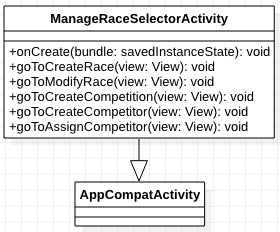
\includegraphics[width=0.4\columnwidth]{manageraceselector_uml.png} 
\caption{Diagramme de classe de ManageRaceSelectorActivity}
\label{fig:manageraceselector_uml}
 \end{figure}

\todo{Image}

\subsection{CreateNewRaceActivity}

L'activité CreateNewRaceActivity permet à l'utilisateur de créer une nouvelle compétition dans la base de données. Une fois que l'utilisateur à rentré toutes les informations, une requête d'insertion est envoyé à la base de données.

La figure \ref{fig:createnewrace_uml} montre le diagramme de classe de CreateNewRaceActivity.

\begin{figure}[htb]
\centering 
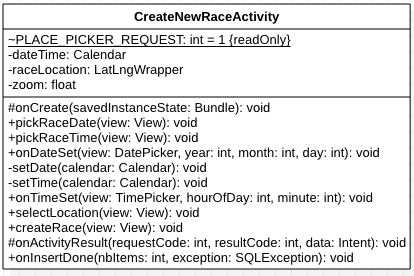
\includegraphics[width=0.6\columnwidth]{createnewrace_uml.png} 
\caption{Diagramme de classe de CreateNewRaceActivity}
\label{fig:createnewrace_uml}
 \end{figure}

\todo{Image}

\subsection{ModifyRaceActivity}

\todo{Image}

\subsection{CreateNewCompetitorActivity}

\todo{Image}

\subsection{AssignCompetitorActivity}

\todo{Image}

\subsection{DatePickerFragment}

Le fragment DataPickerFragment est utilisé pour récupérer une date entrée par l'utilisateur, l'interface habituelle pour entrer une date est présenté à l'utilisateur et son choix est retourné.

La figure \ref{fig:datapickerfragment_uml} montre le diagramme de classe de DatePickerFragment.

\begin{figure}[htb]
\centering 
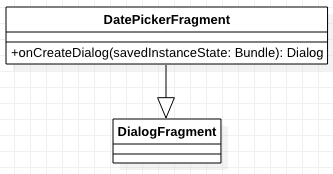
\includegraphics[width=0.5\columnwidth]{datapickerfragment_uml.png} 
\caption{Diagramme de classe de DatePickerFragment}
\label{fig:datapickerfragment_uml}
 \end{figure}

\todo{Image}

\subsection{TimePickerFragment}

Le fragment TimePickerFragment permet la sélection d'une heure, il présente à l'utilisateur l'interface usuelle de sélection de l'heure puis en retourne le choix.

La figure \ref{fig:timepickerfragment_uml} montre le diagramme de classe de TimePickerFragment.

\begin{figure}[htb]
\centering 
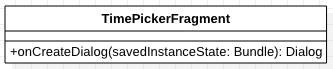
\includegraphics[width=0.5\columnwidth]{timepickerfragment_uml.png} 
\caption{Diagramme de classe de TimePickerFragment}
\label{fig:timepickerfragment_uml}
 \end{figure}

\todo{Image}

\subsection{LatLngWraper}

Cette classe permet d'encapsuler un objet de type LatLng. Cette classe est utilisé pour rendre un objet LatLng serializable.

La figure \ref{fig:latlngwraper_uml} montre le diagramme de classe de LatLngWraper.

\begin{figure}[htb]
\centering 
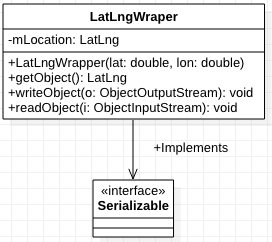
\includegraphics[width=0.4\columnwidth]{latlngwraper_uml.png} 
\caption{Diagramme de classe de LatLngWraper}
\label{fig:latlngwraper_uml}
 \end{figure}

\subsection{OnQueryResultReady}

OnQueryResultReady est une interface que l'utilisateur doit implémenter afin de pouvoir recevoir les résultats des requêtes envoyées à la base de données. La fonction est automatiquement appelé lorsque les résultats de la requête associée sont prêt à être consulté.

La figure \ref{fig:onqueryresultready_uml} montre le diagramme de classe de OnQueryResultReady.

\begin{figure}[htb]
\centering 
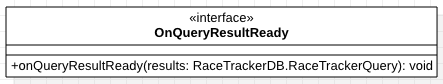
\includegraphics[width=0.6\columnwidth]{onqueryresultready_uml.png} 
\caption{Diagramme de classe de OnQueryResultReady}
\label{fig:onqueryresultready_uml}
 \end{figure}

\subsection{RaceTrackerCompetition}

Cette classe contient les données relatives à une compétition. Elle peut être initialisée directement en lui passant le résultat d'une requête à une base de donnée (ResultSet).

La figure \ref{fig:racetrackercompetition_uml} montre le diagramme de classe de RaceTrackerCompetition.

\begin{figure}[htb]
\centering 
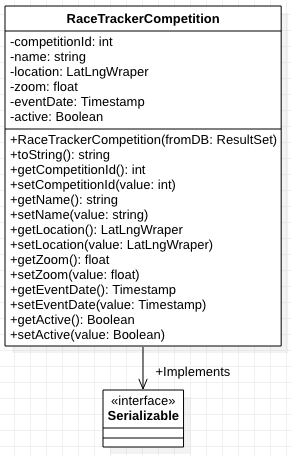
\includegraphics[width=0.5\columnwidth]{racetrackercompetition_uml.png} 
\caption{Diagramme de classe de RaceTrackerCompetition}
\label{fig:racetrackercompetition_uml}
 \end{figure}

\subsection{RaceTrackerCompetitionAdapter}

Cette classe permet de faire la gestion de l'affichage d'une liste d'instance de RaceTrackerCompetition dans un objet de type RecyclerView.

La figure \ref{fig:racetrackercompetitionadapter_uml} montre le diagramme de classe de RaceTrackerCompetitionAdapter.

\begin{figure}[htb]
\centering 
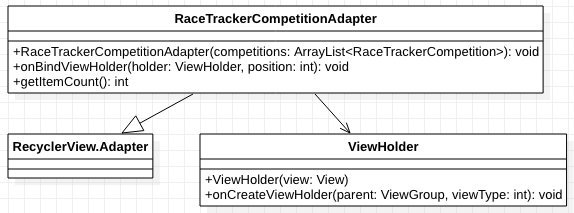
\includegraphics[width=0.8\columnwidth]{racetrackercompetitionadapter_uml.png} 
\caption{Diagramme de classe de RaceTrackerCompetitionAdapter}
\label{fig:racetrackercompetitionadapter_uml}
 \end{figure}

\subsection{RaceTrackerCompetitor}

Cette classe contient les données relatives à un compétiteur. Elle peut être initialisée directement en lui passant le résultat d'une requête à une base de données (ResultSet).

La figure \ref{fig:racetrackercompetitor_uml} montre le diagramme de classe de RaceTrackerCompetitor.

\begin{figure}[htb]
\centering 
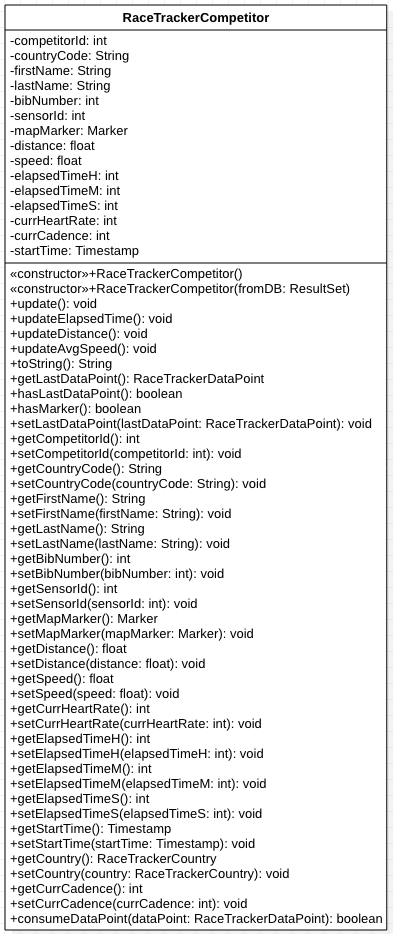
\includegraphics[width=0.5\columnwidth]{racetrackercompetitor_uml.png} 
\caption{Diagramme de classe de RaceTrackerCompetitor}
\label{fig:racetrackercompetitor_uml}
 \end{figure}

\subsection{RaceTrackerCompetitorAdapter}

Cette classe permet de faire la gestion de l'affichage d'une liste d'instance de RaceTrackerCompetitorAdapter dans un objet de type RecyclerView.

La figure \ref{fig:racetrackercompetitoradapter_uml} montre le diagramme de classe de RaceTrackerCompetitorAdapter.

\begin{figure}[htb]
\centering 
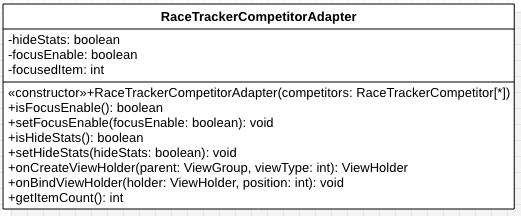
\includegraphics[width=0.8\columnwidth]{racetrackercompetitoradapter_uml.png} 
\caption{Diagramme de classe de RaceTrackerCompetitorAdapter}
\label{fig:racetrackercompetitoradapter_uml}
 \end{figure}

\subsection{RaceTrackerDataPoint}

La classe RaceTrackerDataPoint contient les données relatives à un point de données sur le parcours. C'est ce type de classe que le ViewRaceActivity utilise afin d'afficher à l'utilisateur la position et les informations associées aux coureurs. Elle peut être initialisée directement en lui passant le résultat d'une requête à une base de donnée (ResultSet).

La figure \ref{fig:racetrackerdatapoint_uml} montre le diagramme de classe de RaceTrackerDataPoint.

\begin{figure}[htb]
\centering 
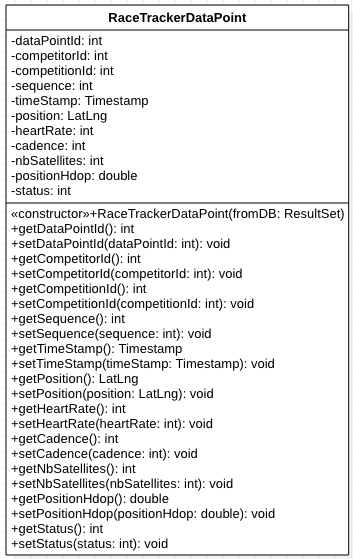
\includegraphics[width=0.4\columnwidth]{racetrackerdatapoint_uml.png} 
\caption{Diagramme de classe de RaceTrackerDataPoint}
\label{fig:racetrackerdatapoint_uml}
 \end{figure}
 
\subsection{RaceTrackerDB}

Le lien entre la base de donnée et l'application mobile, c'est cette classe qui envoie toutes les requête et qui récupère les résultats pour les transmettre, au travers de fonction de callback, à l'utilisateur. C'est cette classe qui fait la gestion du driver JDBC PostgreSQL.

La figure \ref{fig:racetrackerdb_uml} montre le diagramme de classe de RaceTrackerDB.

\begin{figure}[htb]
\centering 
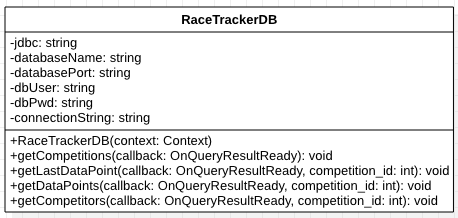
\includegraphics[width=0.6\columnwidth]{racetrackerdb_uml.png} 
\caption{Diagramme de classe de RaceTrackerDB}
\label{fig:racetrackerdb_uml}
 \end{figure}

\todo{Update UML with new methods}

\subsection{RaceTrackerQuery}

Contient une requête pour la base de donnée, son résultat, la fonction de callback de l'utilisateur et éventuellement l'exception si la requête n'a pas pu être exécuté correctement.

La figure \ref{fig:racetrackerquery_uml} montre le diagramme de classe de RaceTrackerQuery.

\begin{figure}[htb]
\centering 
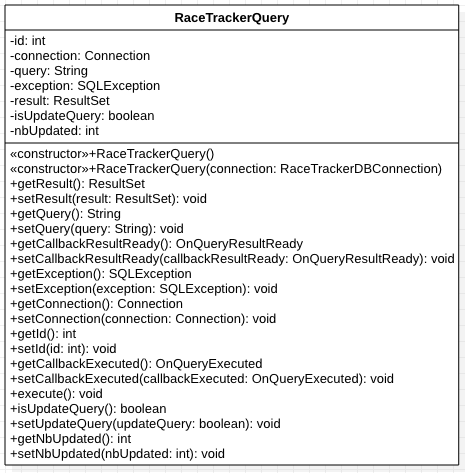
\includegraphics[width=0.4\columnwidth]{racetrackerquery_uml.png} 
\caption{Diagramme de classe de RaceTrackerQuery}
\label{fig:racetrackerquery_uml}
 \end{figure}

\subsection{RaceTrackerDBAsyncTask}

Une classe utilisée par RaceTrackerDB afin d'exécuter une requête de manière asynchrone. En effet il ne faut pas exécuter les requête sur le thread principal car c'est une opération qui prend plusieurs secondes et cela risquerait de bloquer l'exécution de l'application. Afin de pallier à cette effet, on utilise un mécanisme proposé par le système d'exploitation Android et qui permet d'effectuer des tâches en arrière plan et ainsi ne pas bloquer le processus principal.

La figure \ref{fig:racetrackerdbasynctask_uml} montre le diagramme de classe de RaceTrackerDBAsyncTask.

\begin{figure}[htb]
\centering 
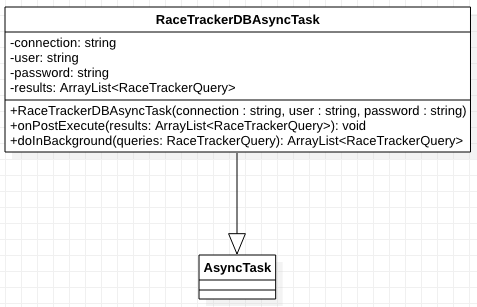
\includegraphics[width=0.6\columnwidth]{racetrackerdbasynctask_uml.png} 
\caption{Diagramme de classe de RaceTrackerDBAsyncTask}
\label{fig:racetrackerdbasynctask_uml}
 \end{figure}

\todo{Nouvelles classes?}